%\documentclass[a4paper, 10pt, twocolumn, journal, twoside]{IEEEtran}
\documentclass[a4paper, 12pt, onecolumn, journal, twoside, draftclsnofoot]{IEEEtran}

\newcommand*{\DOUBLECOL}{}	% turns this on for double column
\newlength{\subfigureheight}
\newlength{\figurewidth}
\ifdefined\DOUBLECOL
\setlength{\subfigureheight}{2.45in}
\setlength{\figurewidth}{3.5in}
\else
\setlength{\subfigureheight}{2.35in}
\setlength{\figurewidth}{6.5in}
\fi
\usepackage[normalem]{ulem} % Use [normalem] to prevent \emph from underlining

\usepackage{amsfonts,amsmath,amssymb,bm,cancel,color,comment,epsfig,enumerate,empheq,floatrow,hyperref,mathdots,mathrsfs}
\usepackage{placeins}%\usepackage{algorithmic}
\usepackage[vlined,ruled,linesnumbered]{algorithm2e}
\usepackage{graphicx}
%\usepackage{amsthm}
\usepackage[super]{nth}
\usepackage[noadjust]{cite}
\usepackage{cancel}

\usepackage{subcaption}
\usepackage{tabularx}
\usepackage{tabularray}		% make thing horizontal lines in tabular
\UseTblrLibrary{booktabs}	% make thing horizontal lines in tabular

\graphicspath{{eps/}}

\hypersetup{
	colorlinks=true,
	linkcolor=red,
	citecolor=green,
	filecolor=magenta,
	urlcolor=blue
}

\newenvironment{Ualgorithm}[1][htpb]{\def\@algocf@post@ruled{\kern\interspacealgoruled\hrule  height\algoheightrule\kern3pt\relax}%
\def\@algocf@capt@ruled{under}
\begin{algorithm}[#1]}
{\end{algorithm}}

\setcounter{MaxMatrixCols}{30}
\DeclareSymbolFont{grb}{OML}{cmm}{b}{it}
\DeclareMathSymbol{\zetab}{\mathord}{grb}{"10}
\DeclareMathSymbol{\etab}{\mathord}{grb}{"11}
\DeclareMathSymbol{\thetab}{\mathord}{grb}{"12}
\DeclareMathSymbol{\kappab}{\mathord}{grb}{"14}
\DeclareMathSymbol{\lambdab}{\mathord}{grb}{"15}
\DeclareMathSymbol{\mub}{\mathord}{grb}{"16}
\DeclareMathSymbol{\nub}{\mathord}{grb}{"17}
\DeclareMathSymbol{\rhob}{\mathord}{grb}{"1A}
\DeclareMathSymbol{\sigmab}{\mathord}{grb}{"1B}
\DeclareMathSymbol{\taub}{\mathord}{grb}{"1C}
\DeclareMathSymbol{\phib}{\mathord}{grb}{"1E}
\DeclareMathSymbol{\psib}{\mathord}{grb}{"20}
\DeclareMathSymbol{\omegab}{\mathord}{grb}{"21}
\DeclareMathSymbol{\epsilonb}{\mathord}{grb}{"22}
\DeclareMathSymbol{\varphib}{\mathord}{grb}{"27}
\input{Symbol_Shortcut.tex}

\SetKwRepeat{Do}{do}{while}%

\newtheorem{theorem}{\bf Theorem}		% by Victor
\newtheorem{corollary}{\bf Corollary}	% by Victor
\newtheorem{definition}{\bf Definition}	% by Victor

%\centerfigcaptionstrue

%\pagestyle{empty}

\makeatletter
\def\ifundefined{\@ifundefined}
\makeatother

\setlength{\parskip}{0ex}

% generating the double accent on o, i.e. \fH{o}, e.g. Erdos Renyi 
\newcommand\fH[1]{\sbox0{#1}\dimen0=\ht0 \advance\dimen0 -1ex
  \sbox2{\'{}}\sbox2{\raise\dimen0\box2}%
  {\ooalign{\hidewidth\kern.1em\copy2\kern-.5\wd2\box2\hidewidth\cr\box0\crcr}}}

\title{\vspace{-0.2em} \huge Latency Minimization for Uplink RSMA System}

\ifdefined \BLIND
\author{Carrson C. Fung $^1$ \\ %and Author 2$^2$ \\
$^1$ NYCU  \\
%email: \emph{Author 1's email, Author 2's email} \\
\thanks{Funding sources.}
}
\else
\author{Shanik Hubert, ~\IEEEmembership{Student Member,~IEEE}, and Carrson C. Fung$^*$,~\IEEEmembership{Member,~IEEE} \\
%Institute of Electronics, College of ECE, National Chiao Tung University, Hsinchu, Taiwan 300 %\\
%Voice: +886-3-573-1862$^2$ Fax: +886-3-572-4361$^2$ email: \emph{rusly.eic04g@nctu.edu.tw, c.fung@ieee.org \vspace{-1.5em}} 
\thanks{This work has been partially supported by Google exploreCSR Grant 111Q90004C.

Shanik Hubert and Carrson C. Fung  are both affiliated with the Department of Electrical and Computer Engineering, National Yang Ming Chiao Tung University, Hsinchu 300, Taiwan. (e-mail: dmytro.ivakhnenkov@gmail.com, c.fung@ieee.org)}
}
\fi


\markboth{IEEE Trans. on Communications}{Latency Minimization for Uplink RSMA System}
\begin{document}
\maketitle

%******************************************************************
\begin{abstract}
%******************************************************************
\end{abstract}

\begin{IEEEkeywords}
\end{IEEEkeywords}

%%%%%%%%%%%%%%%%%%%%%%%%%%%%%%%%%%%%%%%%%%%%%%%%%%%%%%%%%%%%%%%%%%
\section{Introduction}	\label{intro}
%%%%%%%%%%%%%%%%%%%%%%%%%%%%%%%%%%%%%%%%%%%%%%%%%%%%%%%%%%%%%%%%%%


  
%%%%%%%%%%%%%%%%%%%%%%%%%%%%%%%%%%%%%%%%%%%%%%%%%%%%%%%%%%%%%%%%%%
\section{Methodology} \label{sec_meth}
%%%%%%%%%%%%%%%%%%%%%%%%%%%%%%%%%%%%%%%%%%%%%%%%%%%%%%%%%%%%%%%%%%

\subsection{Uplink Blocklength Minimization for Reduction of Asynchronicity}
%******************************************************************
For MIMO uplink (UL), the receive signal is written as
\begin{equation*}
	\y = \sum_{k=1}^K  \H_k \F_k \s_k + \w \in \complex^{N_R},
\end{equation*}
where 
$\H_k \in \complex^{N_R \times N_k}$ denotes the uplink channel between the $k$th user and the AP, $\F_k \in \complex^{N_k \times d_k}$ denotes the precoding matrix for the $k$th user, $d_k$ denotes the number of spatial streams user $k$ is sending to the AP (and $d_k \leq N_k$), $\s_k \in \complex^{d_k}$ denotes the transmitted signal for the $k$th user, $\w \in \complex^{N_R}$  denotes the AWGN, with $N_k$ denoting the number of antennas at the $k$th user and $N_R$ denotes the number of antennas at the AP.  It is assumed that $E \left[ \s_k \s_k^H \right] = \I_{N_k}$.  Let 
\begin{equation*}
	x_k = \F_k \s_k,
\end{equation*}
so
\begin{align*}
	E \left[ \left| \x_k \right\|_2^2 \right] &= \F_k E \left[ \s_k \s_k^H \right] \F_k^H \\
	&= \F_k \F_k^H  \\
	&=  \left\| \F_k \right\|_F^2  \leq P_k,
\end{align*}
where $P_k$ is the transmit power from the $k$th user.  If SIC is used at the receiver, then the achievable rate at the receiver is
\begin{equation*}
	R_{sum} = \sum_{k=1}^K  \log_2 \det \left(  \I_{N_R}  +  \H_k \F_k     \left(  \sigma_w^2 \I_{N_R}  + \sum_{j \neq k}  \H_j \F_j \F_j^H \H_j^H  \right)^{-1}     \F_k^H \H_k^H  \right) 
\end{equation*}

Then it seems the latency minimization problem can be formulated as
\begin{equation}
	\begin{split}
		\min_{\F_k, B_k, \forall k}  &\;  \sum_{k=1}^K  \frac{ B_k } { R_{sum}  }   \text{ ( I think } R_k  \\
		s.t. &\;  \left\| \F_k \right\|_F^2  \leq P_k,  \forall k, \\
		&\; B_k \in \left\{  B_{k,\min}, \ldots, B_{k,\max} \right\},
	\end{split}
\label{eq_prob_form_basic}
\end{equation}
where $R_k$ is the Shannon rate for the $k$th user.  (\ref{eq_prob_form_basic}) makes sense when  infinite size blocklength is assumed.  However, this assumption is usually incorrect when latency is minimized as the design variable should be the number of blocks (i.e. channel used) for transmission, implying the blocklength is short and finite.  Possible extensions for (\ref{eq_prob_form_basic}) include optimizing not with the sum rate, but using rate such as
\begin{enumerate}[1.]
	\item Max-min rate: 
	\begin{equation*}
		\max_{\F_k, \forall k}  \min_k  R_k.
	\end{equation*}
This has a strong fairness guarantee, often leads to equal rates across all users if we can find a feasible solution.  This is the worst-case that Carrson was talking about.
	\item The proportional fairness:
	\begin{equation*}
		\max_{\F_k, \forall k}   \sum_{k=1}^K  \log (\R_k), 
	\end{equation*}
which balances the throughput and fairness. 
	\item Weighted fairness 
	\begin{equation*}
		\max_{\F_k, w_k, \forall k}  w_k \log (R_k), 
	\end{equation*}
where $w_k$ are weights for QoS differentiation, i.e., higher $w_k$ is, more resource will be allocated the $k$th user.
\end{enumerate}


\subsection{Uplink Latency Minimization Using RSMA}
%******************************************************************
Using RSMA for uplink transmission can theoretically acheive the optimal rate region according to \cite{rimoldi1996} by splitting the original $K$ input channels to $2K-1$ inputs (though the $K$th user message need not be split, but most papers consider splitting the last user message for simplicity).  The transmitted message of the $k$th user $\x_k$ is split into 
\begin{equation*}
	\x_k = \sum_{i=1}^2  \\F_{ki} \s_{ki},
\end{equation*}
where $i$ denotes the stream index.  So the received signal at the AP can be written as
\begin{equation*}
	\y = \sum_{k=1}^K \sum_{i=1}^2 \H_{ki} \F_{ki} \s_{ki} + \w \in \complex^{N_R},
\end{equation*}
where
\begin{equation*}
    \sum_{i=1}^2 \left\| \F_{ki} \right\|_F^2  \leq P_k
\end{equation*}

SIC is assumed to be used to decode each user's signal at the AP, which involves the use of a decoding order $\pi$, let the permutation $\pi$ belong to the set $\Pi$ defined as the set of all possible decoding order of all $2K$ messages from $K$ users.  Let the decoding order of message $s_{ki}$ from the $k$th user to be $\pi_{ki}$, then the achievable rate of decoded message $s_{ki}$ can be given as
\begin{equation*}
	\text{\textcolor{red}{missing equation here}.}
\end{equation*}
Let $\mcK$ be the set of user devices, Let $\mcJ = \{1, 2 \}$ be the set of containing the number of split streams.  Then the rate of the $i$th stream for user $k$ is
\begin{equation*}
	R_{ki} = \log_2 \det \left(  \I_{N_R}  +  \H_k \F_{ki}     \left(  \sigma_w^2 \I_{N_R}  + \sum_{\{(j{\in}\mathcal{K},i{\in}\mathcal{J})|\pi_{ji}{>}\pi_{ki}\}}  \H_j \F_{ji} \F_{ji}^H \H_j^H  \right)^{-1}     \F_{ki}^H \H_k^H  \right), 
\end{equation*}
where $\{(j{\in}\mathcal{K},i{\in}\mathcal{J})|\pi_{ji}{>}\pi_{ki}\}$ is the set that represents  the messages $s_{ji}$ that are decoded after  message $s_{ki}$.  Hence the total rate for user $k$ is
\begin{equation*}
    R_k = \sum^2_{i=1} R_{ki}
\end{equation*}
To optimize the rate in uplink RSMA, a joint optimization of both the power management and message decoding order must be done, which results in solving 
%Max-Min Rate
\begin{equation*}
	\begin{split}
		\max_{\F_k, \forall k}  \min_{k, \pi} &\; R_k.  \\
    	\mathrm{s.t.} &\; \sum_{i=1}^2 \left\| \F_{ki} \right\|_F^2  \leq P_k \\
    	&\; \pi \in \Pi, \left\| \F_{ki} \right\|_F^2 \geq  0, \forall k \in \mcK, j \in \mcJ 
    \end{split}
\end{equation*}
This is similar to the optimization problem modeled in \cite{yang2019} where they optimize for the sum rate.


\subsection{Uplink Latency Minimization Using Finite Blocklength Minimzation}
%******************************************************************
To consider latency in URRLC systems with finite blocklength, let us model channel rate not in terms of (bits/s) but as (bits/channel use).  Let blocklength of the $k$th user be $n_k$ or the number of channel used per symbol. Let $T_s$ be the time taken to transmit one symbol.  Then the latency of the $k$th user can be expressed as
\begin{equation*}
	\begin{split}
		\text{Latency}_k &= n_k \times T_s \\ 
		&= \frac{B (\text{bits})}{R\text{(bits/channel use)}} \times T_s (\text{sec})
\end{split}
\end{equation*}
Thus latency for the $k$th user is optimized by optimizing for $n_k$. 

According to \cite{durisi2016}, the \textbf{rate under finite blocklength} is expressed as
\begin{equation}
	R^*(n,\epsilon) = C - \sqrt{\frac{V}{n}}Q^{-1}(\epsilon) + \mathcal{O}\left(\frac{\log n}{n}\right), 
\label{eq_rate_finite}
\end{equation}
where $C$ is Shannon capacity of channel, $Q^{-1}(\cdot)$ is the inverse of the Gaussian $Q$ function, $V$ is the channel dispersion.  According to \cite{durisi2016}, (\ref{eq_rate_finite})  is used to sustain the desired error probability $\epsilon$ for a given packet size $n$, one incurs a penalty on the rate (compared to the channel capacity) that is proportional to $\frac{1}{\sqrt{n}}$.

According to \cite{you2023}, the \textbf{rate under finite blocklength in massive MIMO systems} in high SNR regime is approximated as 
\begin{equation*}
	R_k \approx d_k\log\left(1+\rho_k\right)-\sqrt{\frac{d_k}{n_k}}Q^{-1}\left(\varepsilon_k\right).
\end{equation*}
which is the rate of user $k$.  $\rho_k$ is the SNR of user $k$ and $Q^{-1}(\cdot)$ denotes the inverse of Gaussian $Q$ function.  At this point, we are not sure why \cite{you2023} removed the channel dispersion $V$, which is part of (\ref{eq_rate_finite}).  The inverse of the $Q$ function is  
\begin{equation*}
	Q^{-1}(x) \overset{\Delta}{\operatorname*{=}}\int_{x}^{\infty}\frac{1}{\sqrt{2\pi}}e^{-t^{2}/2} dt.
\end{equation*}
Rearranging the equation, when $d_k$ is large enough, 
\begin{equation*}
    n_k\approx\frac{d_k\left[Q^{-1}\left(\varepsilon_k\right)\right]^2}{\left[d_k\mathrm{log}_2\left(1+\rho_k\right)-R_k\right]^2}\propto\frac{1}{d_k},
\end{equation*}
This shows that the latency in the time domain can be reduced by increasing the DoFs in the space domain, for the purpose of maintaining a certain level of performance target. According to \cite{you2023} 
\begin{equation}
	\begin{split}
    	n_k &= B_k/R_k \\
		&= \frac{B_k}{d_k\log\left(1+\rho_k\right)-\sqrt{\frac{d_k}{n_k}}Q^{-1}\left(\varepsilon_k\right)}. 
	\end{split}
\label{eq_blklength_MIMO}
\end{equation}
Solving (\ref{eq_blklength_MIMO}) would give another equation that describe $n_k$ if we know the number of bits $B_k$. We am not sure how this fits in with the other formulas.  From (\ref{eq_blklength_MIMO}), it can also be seen there are several ways to decrease $n_k$, which are 
\begin{enumerate}
    \item Increase spatial DoF $d_k$
    \item Increase SNR $\rho_k$
    \item Increase error probability $\epsilon_k$ (reliability)
\end{enumerate}

The \textbf{min-max blocklength/Latency} can be expressed as
\begin{equation*}
    \min_{\forall k}  \max_{k,R_k,\epsilon_k, }  n_k. 
\end{equation*}

\subsection{Uplink Latency Minimization with RSMA and Finite Blocklength Minimization}
%******************************************************************
\cite{zhang2023} considered minimizing the blocklength in uplink RSMA in a simple 2-user system. However in our problem, we want to improve the latency of the worst-case user, i.e. the user with the worst channel (e.g. worst channel-to-noise (CNR)), we should consider increasing $d_k$, $\rho_k$, or $\epsilon_k$ of the weakest user through precoder design, while decreasing the same parameters of the stronger users so that all users will experience the same latency, thus reducing asynchronality among the users.   
%
%I feel this has a naturally synergestic approach, as eventhough you increase the error probability of the weaker user, the weighing mechanism in Fed-async takes care to reduce the impact of data from these users on the training.
%
Similarly reducing the error probability of the stronger user will be helpful as the data from teh stronger users are weighted higher. This helps to reduce the unfariness of asynchrononicity and in the context of federated learning, this ensures that the weaker users still have an impact on the training while not weighting the data higher due to higher error rate fro these users due to the poor channel.  This is something that i do not believe is explored in \cite{zhang2023}.

\subsection{Problem Formulation of Blocklength Reduction to Reduce Asynchronality}
%******************************************************************
\textbf{Written  on 8-21-2025.} \\

The Shannon rate of the receiver can be defined as,
\begin{equation*}
	R_{k} =  \log_2 \det \left(  \I_{N_R}  +  \H_k \F_k     \left(  \sigma_w^2 \I_{N_R}  + \sum_{j \neq k}  \H_j \F_j \F_j^H \H_j^H  \right)^{-1}     \F_k^H \H_k^H  \right) 
\end{equation*}
Defining the latency of the $k$th use as 
\begin{equation*}
    T_{k} = \frac{n_k}{f_s}, 
\end{equation*}
where $T_{k}$ is the latency, $n_k \in \mathbb{Z}_+$ is the number of channel used and $f_s$ is the symbol rate.  Considering error probability $\epsilon$ and using the it to calculate latency under the mean no. of retranmsmissions 
\begin{equation*}
    \begin{split}
        &\text{P}(n \ \text{transmissions}) = \epsilon_k^{n-1}(1-\epsilon_k). \\
        &\mathbb{E}( \text{no. of transmissions}) = n_{mean} = \frac{1}{1-\epsilon_k}.
    \end{split}
\end{equation*}
Sincer a finite blocklength $n_k$ is considered, the upper bound to the rate of system for the $k$th user is written as \cite{durisi2016}
\begin{equation*}
	\frac{B_k}{n_k} \leq R_k^*(n, \epsilon) = R_k - \sqrt{\frac{V_k}{n_k}}Q^{-1}(\epsilon_k), 
\end{equation*}
where $B_k$ is the fixed number of bits that need to sent by the $k$th user and $n_k$ is the number of blocklength or channel uses or symbols for the $k$th user. Thus $R_k^*(n, \epsilon)$ can be defined in the unit of (bits/channel use).  Then the weighted latency minimization problem can be formulated as
\begin{equation}
	\begin{split}
		\min_{\F_k, n_k, \epsilon_k} &\; \sum_{k \in K} W_k \frac{n_k}{f_s} \\
		\text{s.t.} &\; \frac{B_k}{n_k} \leq R_k(\F_k) - \sqrt{ \frac{V_k(\F_k)}{n_k} } Q^{-1} (\epsilon_k), \quad \forall k \in \mcK\\
		&\; n_k \in [n_{\text{min}}, n_{\text{max}}], \quad \forall k \in \mcK \\
		& \; \|\F_k\|_F^2 \leq P_k, \quad \forall k \in \mcK.
	\end{split}
\label{eq_short_blocklength_latency_min_prob}
\end{equation}
A more complete formulation by considering user specific $\epsilon_k$ and retransmission affected latency can be considered as
\begin{equation}
	\begin{split}
		\min_{\F_k, n_k, \epsilon_k} &\; \sum_{k \in K} W_k \frac{n_k}{f_s} \frac{1}{1-\epsilon_k} \\
		\text{s.t.} &\; \frac{B_k}{n_k} \le (1-\epsilon_k) \Bigg[ R_k(\F_k) - \sqrt{\frac{V_k(\F_k)}{n_k}} \, Q^{-1}(\epsilon_k) \Bigg], \quad \forall k \in \mcK, \\
		&\; n_k \in [n_{\min}, n_{\max}], \quad \forall k \in \mcK, \\
		&\; \epsilon_k \in [0, \epsilon_0], \quad \forall k \in \mcK, \\
		&\; \|\F_k\|_F^2 \le P_k, \quad \forall k \in \mcK.
	\end{split}
\label{eq_short_blocklength_latency_min__retrans_prob}
\end{equation}


\begin{comment}
\subsection{Applying QoS constraint to the user rate}
%******************************************************************
\textbf{Written on 8-21-2025}\\
This was the original equation which shows the relationship between the user rate $\frac{B_k}{n_k}$ and the theoretical upper limit $R^*(n_k, \epsilon_k) = R_k - \sqrt{\frac{V_k}{n_k}}Q^{-1}(\epsilon_k) $.
\begin{equation*}
    \frac{B_k}{n_k} \leq R_k - \sqrt{\frac{V_k}{n_k}}Q^{-1}(\epsilon_k) \\
\end{equation*}

We then added a QoS bound $\gamma_k$ to give a lower bound to $R^*(n_K,\epsilon_k)$ that is not a function of the variables $n_k$$ as 
\begin{equation*}
     \frac{B_k}{n_k} \leq R_k - \sqrt{\frac{V_k}{n_k}}Q^{-1}(\epsilon_k) \\ \geq \gamma_k
\end{equation*}

This introduces 2 lower bounds for $R^*(n_k \epsilon_k) \geq$  $\frac{B_k}{n_k}$ and $R^*(n_k \_k) \geq$  $\gamma_k$. We know that $\frac{B_k}{n_k}$ is monotonically decreasing in $n_k$, while $R^*(n_k,\epsilon_k)$ is monotonically increasing in $n_k$.  Since the objective is to decrease $n_k$, find an optimal solution such that the equality condition between $\frac{B_k}{n_k}$ and  $R^*(_k)$ is true, i.e.
\begin{equation*}
    \frac{B_k}{n^*_k} = R^*(n^*_k,\epsilon_k) = R_k - \sqrt{\frac{V_k}{n^*_k}}Q^{-1}(\epsilon_k)
\end{equation*}
%let  increase until it meets the decreasing in equality. Now assuming that for the optimal value $n_k^*$ (this is the smallest possible value of $n$ we can get, ie: min latency), 
Then there are 2 cases that must be considered
\begin{enumerate}
    \item Case I: $\gamma_k > R^*(n^*_k,\epsilon_k)$ \\
    In this case, since $\gamma_k > R^*(n^*_k,\epsilon_k)$, $R^*(n^*_k,\epsilon_k)$ is never achieved. \\
    
    As $n_k$ keeps decreasing, $R^*(n_k, \epsilon_k)$ decreases until,
    \begin{equation*}
        R^*(n_k,\epsilon_k) = R_k - \sqrt{\frac{V_k}{n_k}}Q^{-1}(\epsilon_k) = \gamma_k
    \end{equation*}
    Solving for $n_k$
    \begin{equation*}
    n_k = V_k\left(\frac{ Q^{-1}(\epsilon_k)}{R_k - \gamma_k}\right)^2
    \end{equation*}

    This is the minimum blocklength achievable, thus in this case, 
    $n^*_k = V_k \left(\frac{Q^{-1}(\epsilon_k)}{R_k - \gamma_k}\right)^2$
    and maximum user rate = $\frac{B_k}{n^*_k}$

    \item Case II: $\gamma_k < R^*(n^*_k, \epsilon_K) = \frac{B_k}{n^*_k}$ \\
    In this case, $\frac{B_k}{n^*_k}$ provides a lower bound to $R^*(n_k,\epsilon_k)$ before $\gamma_k$. \\

    Thus we believe the equation can be rewritten with $\gamma_k$ acting as a lower bound for $\frac{B_k}{n_k}$ and $R^*(n_k, \epsilon_k)$,
	\begin{equation*}
    	\gamma_k \leq \frac{B_k}{n_k} \leq R^*(n_k, \epsilon_k) = R_k - \sqrt{\frac{V_k}{n_k}}Q^{-1}(\epsilon_k)
	\end{equation*}

    We must solve this to obtain $n^*_k$.
\end{enumerate} 

Solution for (\ref{eq_short_blocklength_latency_min_prob}) can be obtained via alternating optimization.  

We can solve this by first evaluating, 

\begin{equation*}
\begin{split}
    R_k - \sqrt{\frac{V_k}{n_k}}Q^{-1}(\epsilon_k) &= \gamma_k\\
    n^*_k &= V_k \left(\frac{Q^{-1}(\epsilon_k)}{R_k - \gamma_k}\right)^2
\end{split}
\end{equation*}

This is not our final $n^*_k$, once we obtain this $n^*_k$, we substitute it in $\frac{B_k}{n_k}$, \\
\\
if:
\begin{equation*}
    \frac{B_k}{n^*_k} < R_k - \sqrt{\frac{V_k}{n^*_k}}Q^{-1}(\epsilon_k)
\end{equation*}

 then: According to Case I, \\
\begin{equation*}
n^*_k = V_k \left(\frac{Q^{-1}(\epsilon_k)}{R_k - \gamma_k}\right)^2
\end{equation*}
 \\else if: 
\begin{equation*}
    \frac{B_k}{n^*_k}> R_k - \sqrt{\frac{V_k}{n^*_k}}Q^{-1}(\epsilon_k)
\end{equation*}
 
 then: According to Case II, 
 
the inequality of $\frac{B_K}{n_K} \leq R^*(n_k,\epsilon_k)$ is violated, thus to obtain true $n^*_k$ we must solve for,
\begin{equation*}
    \gamma_k \leq \frac{B_k}{n_k} \leq R_k - \sqrt{\frac{V_k}{n_k}}Q^{-1}(\epsilon_k)
\end{equation*}

\textbf{Problem Formulation with QoS constraint}
\begin{equation*}
	\begin{split}
		\min_{F_k, n_k, \gamma_k, \epsilon_k} &\; \sum_{k \in K} W_k \frac{n_k}{f_s} \\
		\text{s.t. } &\; \frac{B_k}{n_k} \le   R_k - \sqrt{\frac{V_k}{n_k}} \, Q^{-1}(\epsilon_k)  \geq \gamma_k, \quad \forall k \in K, \\
		&\; n_k \in [n_{\min}, n_{\max}], \quad \forall k \in K, \\
		&\; \epsilon_k \in [0, \epsilon_0], \quad \forall k \in K, \\
		&\; \|\F_k\|_F^2 \le P_k, \quad \forall k \in K.
	\end{split}
\label{eq_short_blocklength_latency_min_QoS_prob}
\end{equation*}
\end{comment}

\subsection{Strategies to solve the Problem Formulation}
%******************************************************************
Solution for (\ref{eq_short_blocklength_latency_min_prob}) can be attained via alternating optimization.  First, by fixing $\F_k$, $n_k$ can be found via exhaustive search by searching the interval $\left[ n_{\min}, n_{\max} \right]$ for $k \in \mcK$.  Then after a suboptimal (because $n_k$, $\forall k$ is found based on a suboptimal $\F_k$), then fixing $\n_k$, we should find $\F_k$, for $k \in \mcK$, by solving 
\begin{equation}
	\begin{split}
		\max_{\F_k, k \in \mcK} &\; R_k(\F_k) - \sqrt{ \frac{ V_k(\F_k) }{ n_k }  } Q^{-1}(\epsilon_k), \quad \forall k \in \mcK \\
		& \; \left\| \F_k \right\|_F^2 \leq P_k, \quad \forall k \in \mcK.
	\end{split}
\label{eq_latency_min_precoder_subprob}
\end{equation}
This implies if the problem needs to be convex, then $R_k(\F_k)$ needs to be concave (where the maximization of $R_k(\F_k)$ can be done by reformulating the problem into minimization of the WMMSE) and $\sqrt{ \frac{ V_k(\F_k) }{ n_k } }$ needs to be convex.  Since square root is a monotonically nondecreasing concave function, the square root can be removed and $V_k(\F_k)$ can be approximated, e.g. using its first-order Taylor series expansion, so that (\ref{eq_latency_min_precoder_subprob}) can be convexified as
\begin{equation}
	\begin{split}
		\max_{\F_k, k \in \mcK} &\; W_k(\F_k) - \left( V_k \left( \F_k^{(p)} \right) + \nabla V_k \left( \F_k^{(p)} \right)^H  \left( \F_k - \F_k^{(p)} \right) \right), \quad \forall k \in \mcK \\
		& \; \left\| \F_k \right\|_F^2 \leq P_k, \quad \forall k \in \mcK,
	\end{split}
\label{eq_latency_min_precoder_subprob_cvx}
\end{equation}
where $\F_k^{(p)}$ is the precoder at the $p$th iteration of the successive convex optimization (SCA) (or the WMMSE update since the SCA needs to be applied in conjunction with the WMMSE iteration).  

Since the rate of the $k$th user is defined as 
\begin{equation*}
	R_k = \log \det \left(  \I_{N_R}  +  \H_k \F_k  \F_k^H \H_k^H \left(  \sigma_w^2 \I_{N_R}  + \sum_{j \neq k}  \H_j \F_j \F_j^H \H_j^H  \right)^{-1} \right), 
\end{equation*}
let $\H_k \in \complex^{N_r \times N_k}$ with $N_k$ denoting the number of transmit antennas at user $k$.  This implies $\F_k \in \complex^{N_k \times d_k}$, where $d_k \leq N_k$ denotes the number of spatial streams from the $k$th user.  Then it has been shown in \cite{qi2011} that the weighted sum rate
\begin{equation*}
	\sum_{k=1}^K w_k R_k, \quad s.t. \left\| \F_k \right\|_F^2 \leq P_k 
\end{equation*}
can be maximized by solving the WMMSE problem.  Define the $k$th receiver at the AP as $\U_K \in \complex^{N_R \times d_k}$.  Also define the weight matrix $\W_k \in \complex^{d_k \times d_k}$ where $\W_k \succ \0_{d_k \times d_k}$ (which will be equal to $\E_k^{-1}$).  Further define the MSE matrix 
\begin{equation*}
	\E_k \triangleq \I_{d_k} - \U_k^H \H_k \F_k - \F_k^H \H_k^H \U_k + \U_k^H \left( \sigma_w^2 \I_{N_r} + \sum_{j=1}^K \H_j \F_j \F_j^H \H_j^H \right) \U_k \in \complex^{d_k \times d_k}.
\end{equation*}
Then the per user matrix quadratic transform  identity implies
\begin{align*}
	&w_k \log\det\left( \I_{N_R}  +  \H_k \F_k  \F_k^H \H_k^H \left(  \sigma_w^2 \I_{N_R}  + \sum_{j \neq k}  \H_j \F_j \F_j^H \H_j^H  \right)^{-1} \right) \\
	&\quad = \max_{\U_k, \W_k \succ \0_{d_k \times d_k}} \; w_k \left( \log\det \W_k - tr\left(\W_k \E_k\right) \right) + \text{constant}.
\end{align*}
Then the original weighted sum rate prolbme $\displaystyle \max_{\F_k, k \in \mcK} \; w_k R_k$, subject to $\left\| \F_k \right\|_F^2 \leq P_k $ problem is equivalent to 
\begin{equation}
	\begin{split}
		\max_{\F_k, \W_k, \U_k, k \in \mcK} &\; w_k \left( \log\det \W_k - tr\left( \W_k \E_k \right) \right) \\
		s.t. &\; \left\| \F_k \right\|_F^2 \leq P_k.
	\end{split}
\label{eq_WMMSE_equiv_prob}
\end{equation}
Let 
\begin{equation*}
	\bSigma \triangleq \sigma_w^2 \I_{N_R} + \sum_{j=1}^K \H_j \F_j \F_j^H \H_j^H.
\end{equation*}
Then the following WMMSE algorithm can be used to find the solution for (\ref{eq_WMMSE_equiv_prob}).  
\begin{enumerate}[1.]
	\item {\bf MMSE receiver update}
	\begin{equation*}
		\U_k = \bSigma^{-1} \H_k \F_k.
	\end{equation*}
	%
	\item {\bf Weight matrix computation (inverse MSE)}
	\begin{equation*}
		\W_k = \E_k^{-1}
	\end{equation*}
	%
	\item {\bf Precoder computation (quadratic KKT with power constraint)} Let 
	\begin{align*}
		\C_k &\triangleq \H_k^H \U_k \W_k \U_k^H \H_k \in \complex^{N_k \times N_k} \\
		\D_k &\triangleq \H_k^H \U_k \W_k \in \complex^{N_k \times d_k}.
	\end{align*} 
	Then the precoder with per-user power constraint is computed as
	\begin{equation*}
		\F_k(\lambda_k) = \left( \w_k \C_k + \lambda_k \I_{N_k} \right)^{-1}  (\w_k \D_k ) \in \complex^{N_k \times d_k}, 
	\end{equation*}
	where $\lambda_k \geq 0$ is chosen by the bisection method to satisfy $tr\left( \F_k \F_k^H \right) = P_k$ if needed, otherwise $\lambda_k = 0$ and $tr\left( \F_k \F_k^H \right) < P_k$.  That is, this corresponds to the complementary slackness condition in the KKT conditions.
\end{enumerate}
Note that it has been reported that by initializing $\F_k$ using MRT precoder speeds up the convergence of the WMMSE algorithm.  Note also that the sum rate is maximized by maximizing the per-user rate $R_k$.  Note that we may be able to set the weight $w_k$ as the inverse of the CNR so that the rate of the worst-case (i.e. worst CNR) will be optimized the most.  Algorithm \ref{alg_latency_min} summarizes the steps. \\
%**************************************************************************
\begin{algorithm}[H]
	\SetAlgoLined
    \KwResult{$n_k, \; \F_k^\star, \forall k \;$}
    \SetKwInput{Input}{Initialization}
    \Input{Set $i  = 0$, choose $\varepsilon$ (e.g. small integer number), choose $\left\{ \F_k^{(0)}, \forall k \right\}$ as the MRT precoder, $w_k$ = inverse of the $\text{CNR}_k$} %\\
	\Do{ $\displaystyle \left| \sum_{k \in \mcK} n_k^{(i)} - \sum_{k \in \mcK} n_k^{(i-1)} \right| \leq \varepsilon$ }{	
		Exhaustively find $n_k$, $\forall k$ using $\F_k^{(i)}$ \;
		Denote (sub-)optimal blocklength as $n_k^\star$\;
		$n_k^{(i)} = n_k^\star$, $\forall k$ \;
		\For{ each user $k = 1, \ldots, K$ } {
			Use the WMMSE algorithm and convex approximation of $V_k(\F_k)$ to find the precoder $\F_k$ using $n_k^{(i)}$\; 
			Denote (sub-)optimal precoder as $\F_k^\star$\;
    	}
    	$i = i + 1$ \;
    	$\F_k^{(i)} = \F_k^\star$, $\forall k$ \;
    }	
    %$\hbs_W[n|n]=\hbs_W^{(i)}[n|n]$\;
    %$\M[n|n]=\left(\I-\K^{(i-1)}[n]\H \right)\M^{(i-1)}[n|n-1]$\;
    \caption{Proposed latency minimization algorithm in the uplink via precoder.}
\label{alg_latency_min}
\end{algorithm}


%\begin{comment}
%\textbf{Problem Formulation}
%\begin{equation*}
%	\begin{split}
%		\min_{\F_k, n_k, \gamma_k, \epsilon_k} &\; \sum_{k \in K} W_k \frac{n_k}{f_s} \\
%		\text{s.t. } &\; \frac{B_k}{n_k} \le   R_k(\F_k) - \sqrt{\frac{V_k(\F_k)}{n_k}} \, Q^{-1}(\epsilon_k), \quad \forall k \in K, \\
%		&\; n_k \in [n_{\min}, n_{\max}], \quad \forall k \in K, \\
%		&\; \epsilon_k \in [0, \epsilon_0], \quad \forall k \in K, \\
%		&\; \|\F_k\|_F^2 \le P_k, \quad \forall k \in K.
%	\end{split}
%\label{eq_prob_form_basic}
%\end{equation*}
%
%\textbf{Initial Approach (8-21-8-2025)}
%\end{comment}

\subsection{Capacity and Channel Dispersion}
%****************************************************************** 
\textbf{Edited on 29-09-25}

The Capacity and Channel Variance of Coherent Rayleigh Fading Channel is discussed in \cite{collins2019}. 

However \cite{collins2019} makes the folowing assumptions are made,
 
\begin{enumerate}
\item The channel is isotrophic.
\item The noise has unit variance.
\item Considers SU-MIMO.
\end{enumerate}


The Capacity of the channel of user-$k$ is defined as, 

\begin{equation*}
\begin{gathered}
C(P) = \frac{1}{2} \mathbb{E} \Big[ \log \det \big( I_{n_r} + \frac{P}{n_t} \mathbf{H}\mathbf{H}^\dagger \big) \Big] \\
= \sum_{i=1}^{n_{\min}} \mathbb{E} \Big[ C_{\mathrm{AWGN}} \Big( \frac{P}{n_t} \lambda_i^2 \Big) \Big],
\end{gathered}
\end{equation*}

where \( C_{\mathrm{AWGN}}(P) = \frac{1}{2} \log(1+P) \) is the AWGN capacity with unit noise variance, \( n_{\min} = \min(n_r, n_t) \), and \( \lambda_i^2,\, i \in \{1, \ldots, n_{\min}\} \) are the eigenvalues of \( \mathbf{H} \mathbf{H}^\dagger \).


\newpage
\textbf{Channel Variance} 

Assume that $\mathbb{P}[\text{rank} \H > 1] > 0$, then $V (P) = V_{iid}(P)$, 

\begin{equation*}
\begin{aligned}
V_{\mathrm{iid}}(P) &= 
T \, \mathrm{Var} \Bigg( \sum_{i=1}^{n_{\min}} C_{\mathrm{AWGN}}\Big( \frac{P}{n_t} \lambda_i^2 \Big) \Bigg) \\
&\quad + \sum_{i=1}^{n_{\min}} \mathbb{E} \Big[ V_{\mathrm{AWGN}}\Big( \frac{P}{n_t} \lambda_i^2 \Big) \Big] \\
&\quad + \left( \frac{P}{n_t} \right)^2 \left( \eta_1 - \frac{\eta_2}{n_t} \right)
\end{aligned}
\end{equation*}

where \( \lambda_i^2,\, i \in \{1, \ldots, n_{\min}\} \) are the eigenvalues of \( \mathbf{H} \mathbf{H}^H \).

\begin{equation*}
V_{\mathrm{AWGN}}(P) = \frac{(\log e)^2}{2} \left( 1 - \frac{1}{(1+P)^2} \right)
\end{equation*}

\begin{equation*}
\begin{aligned}
& c(\sigma) \triangleq \frac{\sigma}{1 + \frac{P}{n_t} \, \sigma} \\
& \eta_1 \triangleq \frac{(\log e)^2}{2} \sum_{i=1}^{n_{\min}} \mathbb{E} \big[ c^2(\lambda_i^2) \big] \\
& \eta_2 \triangleq \frac{(\log e)^2}{2} \Bigg( \sum_{i=1}^{n_{\min}} \mathbb{E} \big[ c(\lambda_i^2) \big] \Bigg)^2
\end{aligned}
\end{equation*}


\textbf{Obtaining a closed form}

Under high SNR $P \to \infty$. Let $n_{min} = min(n_t,n_r)$, $\alpha = P/n_t$ and $\lambda_i$ the eigenvalues of $\H \H^H$.


\textbf{Reducing} $C_{AWGN}$,

Capacity $C_{AWGN}(x) = \log_e{1+x}$ and in $V_{iid}(P)$, 

%1. 
\begin{equation*}
T\operatorname{Var}\left[\sum_{i=1}^{n_{\min}}C_{\mathrm{AWGN}}(\frac{P}{n_t}\lambda_i^2)\right]=T\operatorname{Var}\left[\sum_{i=1}^{n_{\min}}\ln(1+\alpha\lambda_i^2)\right],\quad\alpha=\frac{P}{n_t}.
\end{equation*}

\begin{equation*}
\operatorname{Var}\!\left[\sum_{i=1}^{n_{\min}} \ln\!\left(1+\alpha \lambda_i^2\right)\right]
\;\sim\;
\operatorname{Var}\!\left[\sum_{i=1}^{n_{\min}} \ln \lambda_i^2 \right]
\end{equation*}

%2. 
\textbf{Reducing} $V_{AWGN}$, 
\begin{equation*}
V_{\mathrm{AWGN}}(P) = \frac{(\log e)^2}{2} \left( 1 - \frac{1}{(1+P)^2} \right)
\end{equation*}

\begin{equation*}
\begin{aligned}
c(\sigma) &\triangleq \frac{\sigma}{1 + \frac{P}{n_t} \, \sigma}, \\
\eta_1 &\triangleq \frac{(\log e)^2}{2} \sum_{i=1}^{n_{\min}} 
           \mathbb{E} \Big[ c^2(\lambda_i^2) \Big], \\
\eta_2 &\triangleq \frac{(\log e)^2}{2} 
           \Bigg( \sum_{i=1}^{n_{\min}} \mathbb{E} \big[ c(\lambda_i^2) \big] \Bigg)^2.
\end{aligned}
\end{equation*}




\begin{equation*}
c(\sigma) \triangleq \frac{\sigma}{1+\frac{P}{n_t}\sigma}, 
\quad \alpha \triangleq \frac{P}{n_t}.
\end{equation*}

\textbf{Reducing} $ (\frac{P}{n_t})^2 (\eta_1-\frac{\eta_2}{n_t})$, 

\textbf{Step 1: High-SNR expansion of $c(\sigma)$}

\begin{equation*}
c(\sigma) = \frac{\sigma}{1+\alpha\sigma} 
= \frac{1}{\alpha}\cdot \frac{1}{1+\tfrac{1}{\alpha\sigma}}.
\end{equation*}

Using the series $\tfrac{1}{1+x} = 1 - x + x^2 + \mathcal{O}(x^3)$ with $x=\tfrac{1}{\alpha\sigma}$:

\begin{equation*}
c(\sigma) = \frac{1}{\alpha} - \frac{1}{\alpha^2\sigma} 
+ \frac{1}{\alpha^3\sigma^2} + \mathcal{O}\!\left(\frac{1}{\alpha^4}\right).
\end{equation*}

---

\textbf{Step 2: Expansion of $\eta_1$}

\begin{equation*}
c(\sigma)^2 = \frac{1}{\alpha^2} - \frac{2}{\alpha^3\sigma} 
+ \mathcal{O}\!\left(\frac{1}{\alpha^4}\right).
\end{equation*}

\begin{equation*}
\eta_1 = \frac{\log^2 e}{2}\sum_{i=1}^{n_{\min}}
\mathbb{E}[c(\lambda_i^2)^2]
= \frac{\log^2 e}{2}\left(
\frac{n_{\min}}{\alpha^2} 
- \frac{2}{\alpha^3}\sum_{i=1}^{n_{\min}}\mathbb{E}\!\left[\tfrac{1}{\lambda_i^2}\right]
+ \mathcal{O}\!\left(\frac{1}{\alpha^4}\right)\right).
\end{equation*}

---

\textbf{Step 3: Expansion of $\eta_2$}

\begin{equation*}
\mathbb{E}[c(\lambda_i^2)] = \frac{1}{\alpha} 
- \frac{1}{\alpha^2}\mathbb{E}\!\left[\tfrac{1}{\lambda_i^2}\right]
+ \mathcal{O}\!\left(\frac{1}{\alpha^3}\right).
\end{equation*}

\begin{equation*}
\sum_{i=1}^{n_{\min}}\mathbb{E}[c(\lambda_i^2)]
= \frac{n_{\min}}{\alpha} 
- \frac{1}{\alpha^2}\sum_{i=1}^{n_{\min}}\mathbb{E}\!\left[\tfrac{1}{\lambda_i^2}\right]
+ \mathcal{O}\!\left(\frac{1}{\alpha^3}\right).
\end{equation*}

\begin{equation*}
\Bigg(\sum_{i=1}^{n_{\min}}\mathbb{E}[c(\lambda_i^2)]\Bigg)^2
= \frac{n_{\min}^2}{\alpha^2} 
- \frac{2n_{\min}}{\alpha^3}\sum_{i=1}^{n_{\min}}\mathbb{E}\!\left[\tfrac{1}{\lambda_i^2}\right]
+ \mathcal{O}\!\left(\frac{1}{\alpha^4}\right).
\end{equation*}

\begin{equation*}
\eta_2 = \frac{\log^2 e}{2}\left(
\frac{n_{\min}^2}{\alpha^2} 
- \frac{2n_{\min}}{\alpha^3}\sum_{i=1}^{n_{\min}}\mathbb{E}\!\left[\tfrac{1}{\lambda_i^2}\right]
+ \mathcal{O}\!\left(\frac{1}{\alpha^4}\right)\right).
\end{equation*}

---

\textbf{Step 4: Reducing $(\frac{P}{n_t})^2 (\eta_1 - \frac{\eta_2}{n_t})$ }
$(\frac{P}{n_t})^2 (\eta_1 - \frac{\eta_2)}{n_t} = \alpha^2 (\eta_1 - \frac{\eta_2}{n_t})$

\begin{equation*}
\eta_1 -\frac{\eta_2}{n_t}= \frac{\log^2 e}{2}\left(
\frac{n_{\min}- \frac{n_{\min}^2}{n_t}}{\alpha^2}
+ \frac{2( \frac{n_{\min}} {n_t} -1)}{\alpha^3}\sum_{i=1}^{n_{\min}}\mathbb{E}\!\left[\tfrac{1}{\lambda_i^2}\right]
+ \mathcal{O}\!\left(\frac{1}{\alpha^4}\right)\right).
\end{equation*}

\begin{equation*}
(\frac{P}{n_t})^2 {n_t}(\eta_1-\eta_2) = \alpha^2(\eta_1-\eta_2/n_t)
= \frac{\log^2 e}{2}\left(
n_{\min}- \frac{n_{\min}^2}{n_t}
+ \frac{ 2( \frac{ n_{\min})} {n_t} -1 } {\alpha}\sum_{i=1}^{n_{\min}}\mathbb{E}\!\left[\tfrac{1}{\lambda_i^2}\right]
+ \mathcal{O}\!\left(\frac{1}{\alpha^2}\right)\right).
\end{equation*}

If we assume that $\alpha \approx \infty$,
\begin{equation*}
 (\frac{P}{n_t})^2(\eta_1- \frac{\eta_2}{n_t})  = \frac{\log^2 e}{2}\left(
n_{\min}-\frac{n_{\min}^2}{n_t}
+ \mathcal{O}\!\left(\frac{1}{\alpha^2}\right)\right)
\end{equation*}
---


\textbf{ Final Value of $ (\frac{P}{n_t})^2 (\eta_1-\frac{\eta_2}{n_t})$}

Having $(\frac{P}{n_t})^2 (\eta_1-\frac{\eta_2}{n_t}))$ to be independant of precoder $\F_k$ by eliminating  $\alpha = \frac{P}{n_t}$, 

\begin{equation*}
 (\frac{P}{n_t})^2 (\eta_1-\frac{\eta_2}{n_t})  = \frac{\log^2 e}{2}\left(
n_{\min}-\frac{ n_{\min}^2 } {n_t}
+ \mathcal{O}\!\left(\frac{1}{\alpha^2}\right)\right)
\quad \text{as } P \to \infty.
\end{equation*}


Having $(\frac{P}{n_t})^2 (\eta_1-\frac{\eta_2}{n_t})$ to be dependant on precoder $\F_k$ by including $\alpha = \frac{P}{n_t}$,

\begin{equation*}
(\frac{P}{n_t})^2 (\eta_1-\eta_2)= \alpha^2(\eta_1-\eta_2/n_t)
= \frac{\log^2 e}{2}\left(
n_{\min}- \frac{n_{\min}^2}{n_t}
+ \frac{ 2( \frac{ n_{\min})} {n_t} -1 } {\alpha}\sum_{i=1}^{n_{\min}}\mathbb{E}\!\left[\tfrac{1}{\lambda_i^2}\right]
+ \mathcal{O}\!\left(\frac{1}{\alpha^2}\right)\right).
\end{equation*}




%3.
\textbf{Reducing}  $T\,\mathrm{Var}\!\left[\sum_{i=1}^{n_{\min}}\ln \lambda_i^2\right]$,

We can further expand $T\,\mathrm{Var}\!\left[\sum_{i=1}^{n_{\min}}\ln \lambda_i^2\right]$ with the trigamma function $\psi1(x)$

\begin{equation*}
\begin{aligned}
\mathrm{Var}\!\left[\sum_{i=1}^{n_{\min}}\ln \lambda_i^2\right] 
&= \sum_{i=1}^{n_{\min}} \psi_1(n_{\max}-i+1),\\
&\quad n_{\min} = \min(n_t,n_r), \quad n_{\max} = \max(n_t,n_r),\\
&\quad \alpha = \frac{P}{n_t}
\end{aligned}
\end{equation*}

where $\psi_1(x)$ is, 
\begin{equation*}
\psi_1(x)=\sum_{k=0}^\infty\frac{1}{(x+k)^2}.
\end{equation*}

In the assumtption of very large $x$, 
\begin{equation*}
\psi_1(x)=\frac{1}{x}+\frac{1}{2x^2}+\frac{1}{6x^3}-\frac{1}{30x^5}+\frac{1}{42x^7}-\cdots
\end{equation*}

Thus when we consider $\sum_{i=1}^{n_{\min}} \psi_1(n_{\max}-i+1)$ to obtain a closed form for the trigamma function, we need to assume a very large $n_{\max}-i+1$, thus if $n_{\max} = \max(n_r,n_t) \to \infty$, 

\begin{equation*}
\begin{split}
\psi_1(n_{\max}-i+1)
&= \frac{1}{n_{\max}-i+1}
+ \frac{1}{2(n_{\max}-i+1)^2} \\
&\quad+ \frac{1}{6(n_{\max}-i+1)^3}
- \frac{1}{30(n_{\max}-i+1)^5}
+ \cdots
\end{split}
\end{equation*}


or using the Bernoulli numbers $B$,
\begin{equation*}
\psi_1(n_{\max}-i+1) = \sum_{k=0}^\infty\frac{B_{2k}}{(n_{\max}-i+1)^{2k+1}}
\end{equation*}

Thus we can reduce $\mathrm{Var}\!\left[\sum_{i=1}^{n_{\min}}\ln \lambda_i^2\right] $ to, 

\begin{equation*}
\mathrm{Var}\left[\sum_{i=1}^{n_{\min}}\ln\lambda_i^2\right]\approx\sum_{i=1}^{n_{\min}}\psi_1(n_{\max}-i+1)=\sum_{i=1}^{n_{\min}}\left[\frac{1}{n_{\max}-i+1}+\frac{1}{2(n_{\max}-i+1)^2}\right.+ \cdots
\end{equation*}

\textbf{Final closed form for Channel Variance}

Thus the final $V(P)$ under the assumption of, $P \to \infty$ and $n_{\max} \to \infty$ is, 

Case 1: when $V(P)$ is independent on precoder $\F_k$,
 \begin{equation*}
\begin{aligned}
V(P) \;=\; V_{\mathrm{iid}}(P) 
&\;\approx\; \; \sum_{i=1}^{n_{\min}}\!\left[
    \frac{1}{\,n_{\max}-i+1\,}
    + \frac{1}{2(n_{\max}-i+1)^2}
    + \cdots
\right] \\[0.6em]
&\quad +\; n_{\min}(\ln e)^2 \\[0.6em]
&\quad +\; \frac{\log^2 e}{2}\left(
n_{\min}-\frac{ n_{\min}^2 } {n_t}
+ \mathcal{O}\!\left(\frac{1}{\alpha^2}\right)\right)
\quad \alpha=\tfrac{P}{n_t}.
\end{aligned}
\end{equation*}

Case 2:  when $V(P)$ is dependent on precoder $\F_k$,
\begin{equation*}
\begin{aligned}
V(P) \;=\; V_{\mathrm{iid}}(P) 
&\;\approx\; \; \sum_{i=1}^{n_{\min}}\!\left[
    \frac{1}{\,n_{\max}-i+1\,}
    + \frac{1}{2(n_{\max}-i+1)^2}
    + \cdots
\right] \\[0.6em]
&\quad +\; n_{\min}(\ln e)^2 \\[0.6em]
&\quad +\; \frac{\log^2 e}{2}\left(
n_{\min}- \frac{n_{\min}^2}{n_t}
+ \frac{ 2( \frac{ n_{\min})} {n_t} -1 } {\alpha}\sum_{i=1}^{n_{\min}}\mathbb{E}\!\left[\tfrac{1}{\lambda_i^2}\right]
+ \mathcal{O}\!\left(\frac{1}{\alpha^2}\right)\right).
\quad \alpha=\tfrac{P}{n_t}.
\end{aligned}
\end{equation*}

\subsection{Revised Uplink Blocklength Minimization for Reduction of Asynchronicity in Rayleigh Fading Channel}
%**************************************************************************
\textbf{Edited on 29-09-25}

In the classical infinite blocklength regime, the achievable rate of a user in a MIMO uplink channel is characterized by the Shannon capacity expression
\begin{equation*}
	R_k = \log \det \left(  \I_{N_R}  +  \H_k \F_k  \F_k^H \H_k^H \left(  \sigma_w^2 \I_{N_R}  + \sum_{j \neq k}  \H_j \F_j \F_j^H \H_j^H  \right)^{-1} \right), 
\end{equation*}
where $\H_k$ denotes the channel matrix of the $k$th user, $\F_k$ is the precoding matrix and $\sigma_w^2 $the noise variance. This formulation assumes that the blocklength, i.e., the number of channel uses for transmitting a codeword, tends to infinity, which enables arbitrarily small error probability through sufficiently long channel codes.  This is illustrated in Fig. \ref{fig_symbol_blklength}
%******************************************************************
\begin{figure}[t]
\centering
	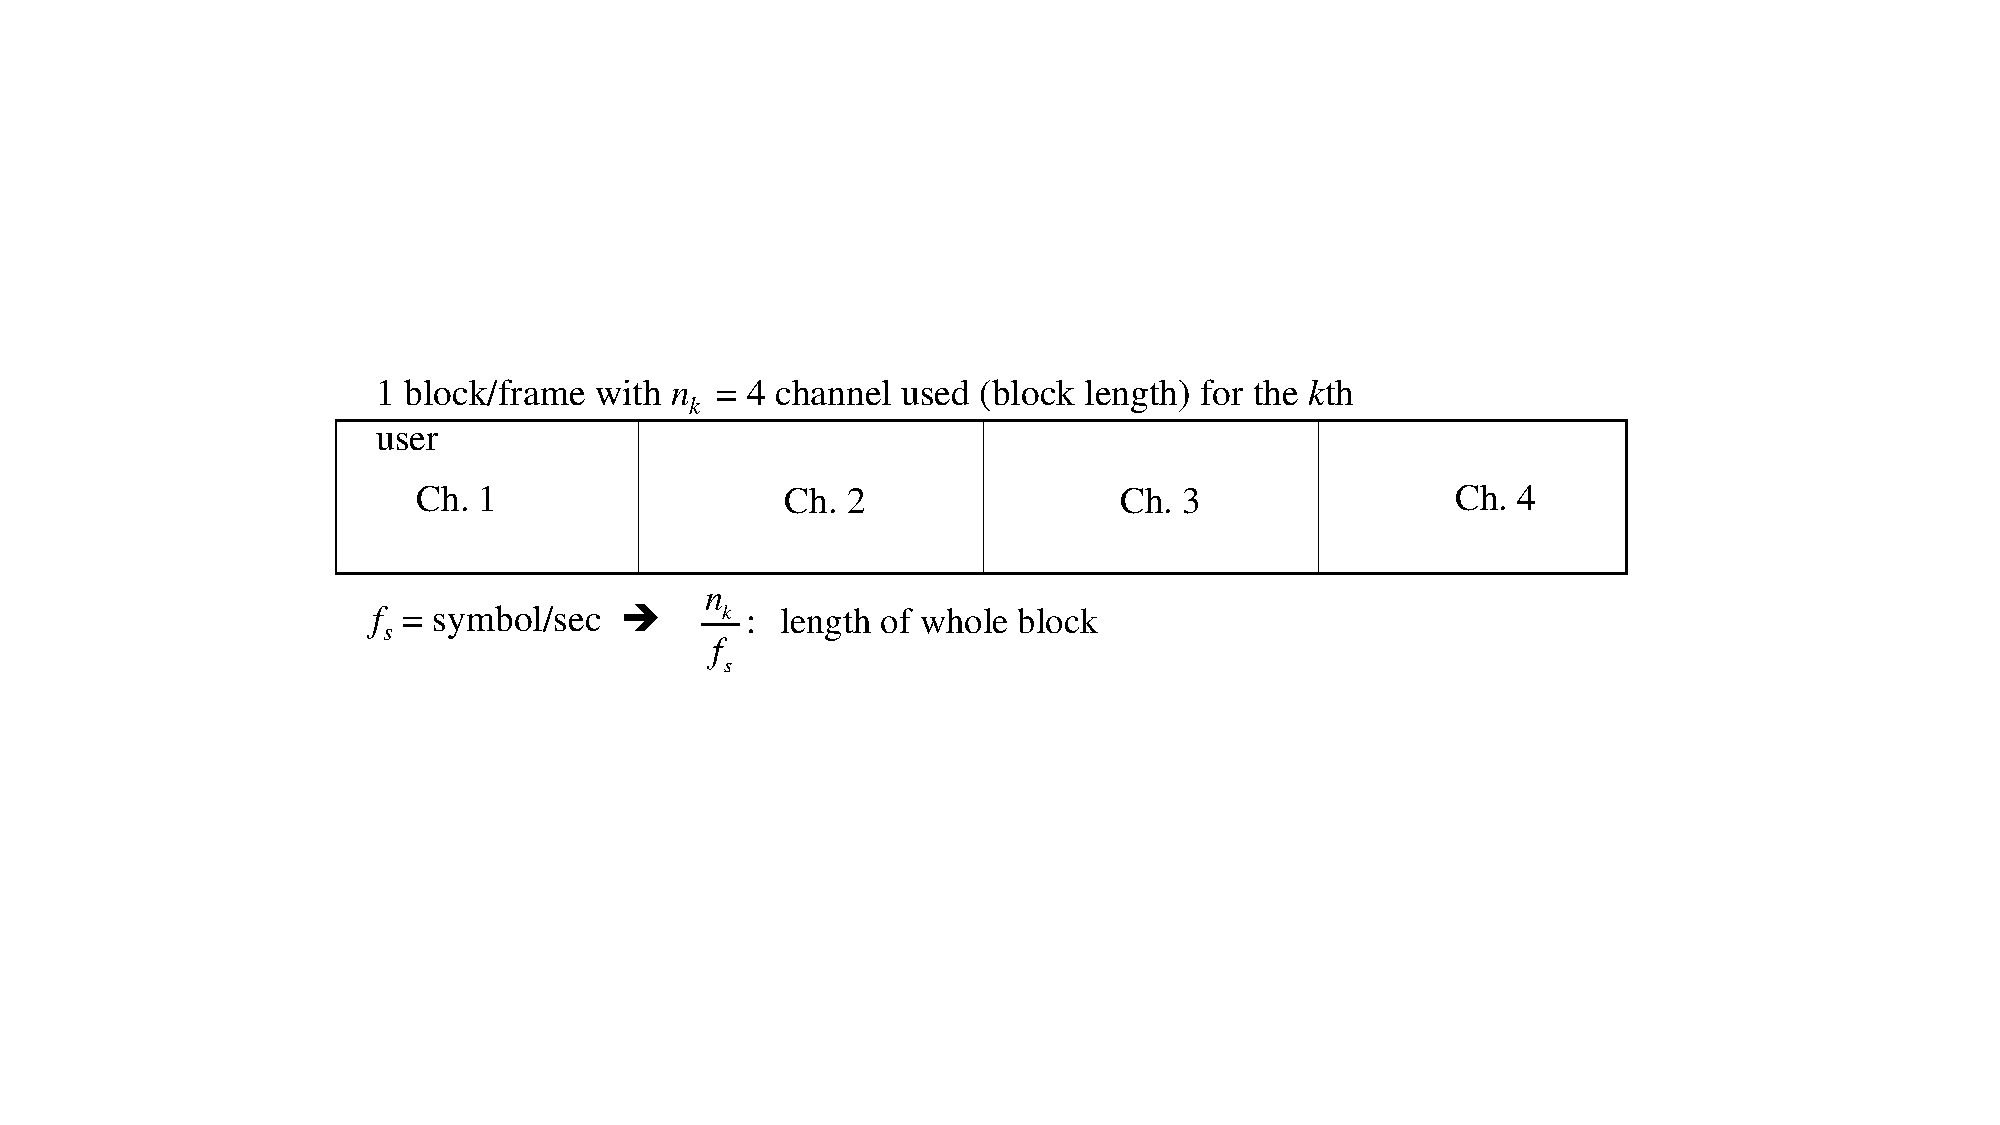
\includegraphics[width = 0.9\columnwidth]{figs/fig_symbol_blklength.pdf} 
	\caption{Illustration of blocklength (or channel used) in a block/frame of bits.  The figure shows that $n_k = 4$, so $\frac{n_k}{f_s}$ denotes the length of the whole block/frame in time (sec).} 
\label{fig_symbol_blklength}
\end{figure}
%******************************************************************

In reality most low latency application operate in the finite blocklength regime, where the number of transmitted symbols $n$ is limited. In this case in a Gaussian channel, the received signal with blocklength $n$ can be written as
\begin{equation*}
	\Y = \sum_{k=1}^K \H_K \F_k  \S_k + \W
\end{equation*}
where the received signal $\Y \in \mathbb{C}^{N_R \times n}$, the transmitted signal $\S_k \in \mathbb{C}^{d_k \times n}$, the Gaussian channel matrix $\H_k \in \mathbb{C}^{N_R \times N_k}$, the precoder matrix $\F \in \mathbb{C}^{ N_k \times d_k}$, the noise matrix $\W \in \mathbb{C}^{N_R \times n}$  and $d_k \leq N_k$.  $N_k$ denotes the number of transmitted antenna at the $k$th user.
 
However this assumes a fixed Gaussian channel, a time-varying Rayleigh fading will be considered herein. Let $T$ denote the coherence time of the channel, i.e. the number of channel uses over which the channel remains constant.  Then the blocklength (total channel uses) of a codeword can be written as
\textcolor{red}{THIS EQUATION STILL DOESN'T MAKE SENSE TO ME.  If $T$ is the channel used/coherent interval, then it should always be 1 as 1 channel used occupies 1 coherent interval}
\begin{equation*}
	n = L \times T
\end{equation*}
where $T$ is the number of channel uses over which the channel remains constant and $L$ is the number of coherent channels within one blocklength.

By considering the coherent intervals, the received signal can be written as \\
\textcolor{blue}{From now on, don't use ``l'', because that will be confused as ``1'' (one).  Use $\ell$ instead}
\begin{equation*}
	\Y = \sum_{k=1}^K \sum_{\ell = 1}^L \H_{k, } \F_{k, \ell}  \S_{k, \ell} + \W \ \in \complex^{L \times N_r \times T}
\end{equation*}
where $\Y \in \complex^{L \times N_r \times T}$, $\H_k \in \complex^{L \times N_r \times N_k}$, $\F_k \in \complex^{L \times N_k \times d_k}$, $\S_k \in \complex^{L \times d_k \times T}$

\text{\sout{(i think it can also be written as 
$Y \in \complex^{N_r \times L \times T}$, 
$\H_k \in \complex^{N_r \times L \times N_k}$, 
$\F_k \in \complex^{N_k \times L \times d_k}$, 
$\S_k \in \complex^{d_k \times L \times T}$)}}

\subsection{Problem Formulation with Rayleigh Fading Channel}
%**************************************************************************
Let $B_k$ be number of bits sent by the $k$th user, let $n_k$ be the blocklength of user $k$, let $\F_k$ be the precoder of user-$k$.  Let blocklength of user $k$ be split in coherent intervals as 
\textcolor{red}{SAME HERE. THIS EQUATION STILL DOESN'T MAKE SENSE TO ME.  If $T_K$ is the channel used/coherent interval, then it should always be 1 as 1 channel used occupies 1 coherent interval}
\begin{equation*}
	n_k = L_k \times T_K
\end{equation*}
where $L_k$ is the number of coherent intervals within the blocklength of user $k$ (cf. Fig. \ref{fig_symbol_blklength}, this can mean  bv) and $T_k$ is the number of channel uses in one coherent interval of user $k$.

A weighted latency minimization problem can be defined as 
\begin{equation}
	\begin{split}
		\min_{\F_{k,\ell}, n_k, \epsilon_k} \;& \sum_{k \in K} w_k \frac{n_k}{f_s} \\
		\text{s.t.}\;& \frac{B_k}{n_k} \leq \max_{\F_{k, \ell}} \frac{1}{L_k} \sum_{l=1}^{L_k} R^*(T_{k}, \F_{k, \ell}), \quad \forall k \in \mcK \\ 
		& n_k \in [n_{\text{min}}, n_{\text{max}}], \quad \forall k \in \mcK \\
		& \|\F_{k,\ell}\|_F^2 \leq P_{k,\ell}, \quad \forall \ell \in [0, L_k],  \forall k \in \mcK,
	\end{split}
\label{eq_short_blocklength_latency_min_prob}
\end{equation}
where the finite blocklength rate for coherent interval $\ell$ of user $k$ is defined as, 
\begin{equation*}
R^*(T_{k} , \F_{k,\ell}) =  C_k(\F_{k,\ell}) - \sqrt{ \frac{V_k(\F_{k,\ell})}{ T_{k, \ell} } } Q^{-1}  (\epsilon_k), \quad \forall \ell \in [0,L_k] \forall k \in \mcK\\
\end{equation*}
The channel variance of the $k$th user in coherence interval $\ell$ is defined as, 
\begin{equation*}
	\begin{aligned}
		V_k(P_{k,\ell}) 
		&\;\approx\; \sum_{i=1}^{N_{k, \min}} \Bigg[
    	\frac{1}{\,N_{k, \max}-i+1\,}
    		+ \frac{1}{2 (N_{k, \max}-i+1)^2}
    		+ \dots
		\Bigg] \\[0.6em]
		&\quad + N_{k, \min} (\ln e)^2 \\[0.6em]
		&\quad + \frac{(\ln e)^2}{2} \Bigg(
		N_{k, \min} - \frac{N_{k, \min}^2}{N_k}
		+ \frac{2 \Big( \frac{N_{k, \min}}{N_k} - 1 \Big)}{\alpha_{k,\ell}} 
        \sum_{i=1}^{N_{k, \min}} \mathbb{E} \Big[ \frac{1}{\lambda_{k, \ell, i}^2} \Big]
		+ \mathcal{O}\Big( \frac{1}{\alpha_{k,\ell}^2} \Big)
		\Bigg), \\[0.6em]
	\end{aligned}
\end{equation*}
where $\alpha_{k,\ell} = \frac{P_{k,\ell}}{N_k}$ is the SNR and $P_{k,\ell}$ is the transmit power. However since we are assuming an isotrophic Raylegh fading channel it is also equal to the total transmit power thus, $P_{k,\ell} = \|\F_{k,\ell}\|_F^2 $.


\subsection{Solution in case of Rayleigh Fading Channel}
%******************************************************************
\begin{equation}
	\begin{split}
		\min_{\F_{k,\ell}, n_k, \epsilon_k} \;& \sum_{k \in K} w_k \frac{n_k}{f_s} \\
		\text{s.t.}\;& \frac{B_k}{n_k} \leq \max_{\F_{k, \ell}} \frac{1}{L_k} \sum_{\ell=1}^{L_k} 		R^*(T_{k}, \F_{k, \ell}), \quad \forall k \in \mcK \\ 
		& n_k \in [n_{\text{min}}, n_{\text{max}}], \quad \forall k \in \mcK \\
		& \|\F_{k,\ell}\|_F^2 \leq P_{k,\ell}, \quad \forall \ell \in [0, L_k],  \forall k \in \mcK.
	\end{split}
\label{eq_short_blocklength_latency_min_prob}
\end{equation}
(\ref{eq_short_blocklength_latency_min_prob}) can be solved by first fixing $\F_{k,\ell}$ and finding $n_k$ via exhaustive search between $[n_{min}, n_{max}]$.  This is followed by fixing $n_k$ to the value that was found in the previous step and maximizing $R^*(T_k, \F_{k,\ell})$ to reduce the latency by increasing the upper bound in the 1st constraint of (\ref{eq_short_blocklength_latency_min_prob}). 

To convert  $R^*(T_k, \F_{k,\ell})$ into a concave function, the square root in $\sqrt{\frac{V(\F_{k,\ell})}{T_k}} Q^{-1}{(\epsilon_k)}$ is removed, followed by variable substitution by solving $\Q_{k,\ell} \triangleq \F_{k,\ell}\F_{k,\ell}^H$ instead of $\F_{k,\ell}$.  This makes $R^*(T_k, \Q_{k,\ell})$ a concave function. Then $R^*(T_k, \Q_{k,\ell})$ is maximized as 
\begin{equation}
	\begin{split}
		\max_{\F_{k,\ell} \in \mcC}  \; C_k(\F_{k,l}) - V(\F_{k,\ell}) 
&=  \max_{\F_{k,\ell} \in \mcC} \; \log \det \Big( \sigma_w^{-2} \H_{k,\ell} \F_{k,\ell} \F_{k,\ell}^H \H_{k,\ell}^H \Big)
   - \frac{V(\F_{k,\ell})}{T_k} Q^{-1}(\epsilon_k),
%&= - \min_{\Q_{k,\ell} \succeq 0} \; - \log \det \Big( \sigma_w^{-2} \H_{k,\ell} \Q_{k,\ell} \H_{k,\ell}^H \Big)
   - \frac{V(\Q_{k,\ell})}{T_k} Q^{-1}(\epsilon_k)
	\end{split}
\label{eq_max_rate}
\end{equation}
where $\displaystyle \mcC = \left\{ \F_{k,\ell} \left| \frac{B_k}{n_k} \leq \max_{\F_{k, \ell}} \frac{1}{L_k} \sum_{\ell=1}^{L_k} R^*(T_{k}, \F_{k, \ell}),   \|\F_{k,\ell}\|_F^2 \leq P_{k,\ell}, \forall \ell \in [0, L_k], \text{for } k = 1, \ldots K,   \right. \right\}$.  
The solution for both $n_k$ and $\Q_{k,\ell}$ is obtained through alternating optimization by solving (\ref{eq_short_blocklength_latency_min_prob}) and (\ref{eq_max_rate}).  Once the optimal $\Q_{k,\ell}$ is obtained, $\F_{k,\ell}$ can be found via a randomization procedure that satisfies the transmit power constraint $\|\F_{k,\ell}\|_F^2 \leq P_{k,\ell}$, $\forall \ell \in [0, L_k],  \forall k \in \mcK$ as outlined in \cite{chang2015semm}.

Since it appears to is difficult to convexify (\ref{eq_max_rate}) due to the complex nature of $V(\F_{k,\ell})$, (\ref{eq_short_blocklength_latency_min_prob}) can be solved using a neural network.  Finding $n_k$ is the same as before, i.e. using exhaustive search.  However, solving for (\ref{eq_max_rate}) will be different.  Since the problem is a constrained problem, its Lagrangian can be written as
\begin{equation*}
	\mcL (\F_{k,\ell}, \lambda_1, \lambda_2) = R^*(T_k, \F_{k,\ell}) + \lambda_1 \left( R^*(T_k, \F_{k,\ell}) - \frac{B_k}{n_k} \right) + \lambda_2 \left( P_{k,\ell} - tr\left(\F_{k,\ell} \F_{k,\ell}^H \right) \right).
\end{equation*}
(\ref{eq_max_rate}) can be solved via the primal-dual algorithm by breaking it into the following three problems
\begin{subequations}
	\begin{align}
		\F_{k,\ell}^{(i+1)} &= \argmax_{\F_{k,\ell}^{(i)}} \; \mcL (\F_{k,\ell}^{(i)}, \lambda_1^{(i)}, \lambda_2^{(i)})	\label{eq_F_soln} \\
		\lambda_1^{i+1} &= \argmin_{\lambda_1} \; \mcL (\F_{k,\ell}^{(i+1)}, \lambda_1, \lambda_2^{(i)})	\nonumber \\
		&= \left[ \lambda_1^{(i)}  - \eta_{\lambda_1}^{(i)} \left( R^*(T_k, \F_{k,\ell}^{(i+1)}) - \frac{B_k}{n_k^{(i+1)}} \right) \right]_+ 	\label{eq_lambda1_soln}	\\
		\lambda_2^{(i+1)} &= \argmin_{\lambda_2} \; \mcL (\F_{k,\ell}^{(i+1)}, \lambda_1^{(i+1)}, \lambda_2) \nonumber \\
		&=  \left[  \lambda_2^{(i)} - \eta_{\lambda_2}^{(i)} \left( P_{k,\ell} - tr\left(\F_{k,\ell}^{i+1} \F_{k,\ell}^{(i+1) \; H} \right) \right) \right]_+.
			\label{eq_lambda2_soln}
	\end{align}
	\label{eq_soln}
\end{subequations}
According to the complementary slackness condition, 
\begin{align*}
	\lambda_1 \left( R^*(T_k, \F_{k,\ell}) - \frac{B_k}{n_k} \right) &= 0 \\
	\lambda_2 \left( P_{k,\ell} - tr\left(\F_{k,\ell} \F_{k,\ell}^H \right) \right) &= 0, 
\end{align*}
which implies that either $\lambda_1 = 0$ or $R^*(T_k, \F_{k,\ell}) - \frac{B_k}{n_k} = 0$ and $\lambda_2 = 0$ or $P_{k,\ell} - tr\left(\F_{k,\ell} \F_{k,\ell}^H \right) = 0$ when the primal-dual algorithm converges.  The iteration should be terminated using the above complementary slackness conditions, as well as the other relevant KKT conditions.

(\ref{eq_F_soln}) can be solved by parameterizing the solution using a neural network with parameters $\btheta$ so that it can be found using gradient ascent
\begin{equation}
	\btheta_{k, \ell}^{(i+1)} = \btheta_{k, \ell}^{(i)} + \eta_{\btheta_{k,\ell}}^{(i)} \nabla_{\btheta_{k,\ell}^{(i)}}  \mcL (\btheta_{k,\ell}^{(i)}, \lambda_1^{(i)}, \lambda_2^{(i)}),
\label{eq_F_soln_NN}
\end{equation}
here the input to the model is the channel, the output is the precoder $\F_{k,\ell}^{(i+1)}$.  That is,  $\F_{k,\ell}^{(i)} = f\left( \h^{(i)}; \btheta_{k,\ell}^{(i)} \right)$, with $f(\cdot)$ denoting the output of the neural network parameterized by $\btheta_{k,\ell}^{(i)}$, with input $\h^{(i)}$ (the channel at the $i$th iteration).  The step sizes $\eta_{\btheta_{k,\ell}}^{(i)}$, $\eta_{\lambda_1}^{(i)}$, and $\eta_{\lambda_2}^{(i)}$ may be obtained using backtracking line search, exponential decaying sequence, or something else that decays as the iteration index $i$ increases.  Reference \cite{shi2021} and reference therein for more information about what choice of neural network you should use.

Hence, the algorithm first finds $\F_{k,\ell}^{(i+1)}$ by solving (\ref{eq_F_soln_NN}) by fixing $\lambda_1$ and $\lambda_2$ to be $\lambda_1^{(i)}$ and $\lambda_2^{(i)}$, respectively.  After obtaining $\F_{k,\ell}^{(i+1)}$, then $\lambda_1^{(i+1)}$ will be obtained using (\ref{eq_lambda1_soln}).  Finally, $\lambda_2^{(i+1)}$ will be obtained using (\ref{eq_lambda2_soln}).  Since it is $\displaystyle \frac{1}{L_k} \sum_{\ell=1}^{L_k} 		R^*(T_{k}, \F_{k, \ell})$ that needs to be maximized, variables need to be solved for all $\ell = 1, \ldots, L_k$ and $k = 1, \ldots K$.  



\subsection{Reformulating in AWGN to simplify channel dispersion}

Since precoder $\F$ was not included in Rayleigh Fading channel dispersion equation $V_{iid}(P)$ we will consider an AWGN channel for simplicity.

\begin{equation*}
	\y = \sum_{k=1}^K \F_k \s_k + \w \in \complex^{N_R},
\end{equation*}
where 
$\F_k \in \complex^{N_k \times d_k}$ denotes the precoding matrix for the $k$th user, $d_k$ denotes the number of spatial streams user $k$ is sending to the AP (and $d_k \leq N_k$), $\s_k \in \complex^{d_k}$ denotes the transmitted signal for the $k$th user, $\w \in \complex^{N_R}$  denotes the AWGN, with $N_k$ denoting the number of antennas at the $k$th user and $N_R$ denotes the number of antennas at the AP.  It is assumed that $E \left[ \s_k \s_k^H \right] = \I_{N_k}$.


The optimization problem then becomes, 

\begin{equation*}
	\begin{split}
		\min_{\F_{k,\ell}, n_k, \epsilon_k} \;& \sum_{k \in K} w_k \frac{n_k}{f_s} \\
		\text{s.t.}\;& \frac{B_k}{n_k} \leq \max_{\F_{k, \ell}} \frac{1}{L_k} \sum_{\ell=1}^{L_k} 		R^*(T_{k}, \F_{k, \ell}), \quad \forall k \in \mcK \\ 
		& n_k \in [n_{\text{min}}, n_{\text{max}}], \quad \forall k \in \mcK \\
		& \|\F_{k,\ell}\|_F^2 \leq P_{k,\ell}, \quad \forall \ell \in [0, L_k],  \forall k \in \mcK.
	\end{split}
	%\label{eq_short_blocklength_latency_min_prob}
\end{equation*}

where $R^*(T_k, \F_{k,\ell})$ is,

\begin{equation*}
	R^*(T_{k} , \F_{k,\ell}) =  C_{k,l}(\F_{k,\ell}) - \sqrt{ \frac{V_k(\F_{k,\ell})}{ T_{k, \ell} } } Q^{-1}  (\epsilon_k), \quad \forall \ell \in [0,L_k] \forall k \in \mcK\\
\end{equation*}

The Capacity and Channel Dispersion equation can be for AWGN MIMO can be derived from \cite{yuri2010} which presents the equations with SNR $\rho$.
\begin{equation*}
	\begin{aligned}
		\mathbf{A}_{k,\ell}(\mathbf{F}_{k,\ell}) &= \sigma^{-2} \mathbf{H}_{k,\ell} \mathbf{F}_{k,\ell} \mathbf{F}_{k,\ell}^H \mathbf{H}_{k,\ell}^H, \\[2mm]
		C_{k,\ell}(\mathbf{F}_{k,\ell}) &= \log_2 \det \Big( \mathbf{I} + \mathbf{A}_{k,\ell}(\mathbf{F}_{k,\ell}) \Big), \\[1mm]
		V_{k,\ell}(\mathbf{F}_{k,\ell}) &= \sum_i \frac{\lambda_i \left(\lambda_i + 2 \right)}{\left(\lambda_i + 1 \right)^2} (\log_2 e)^2 \\[1mm]
		&= \text{tr} \Big[ \mathbf{A}_{k,\ell} (\mathbf{A}_{k,\ell}+2 \mathbf{I}) (\mathbf{A}_{k,\ell} + \mathbf{I})^{-2} \Big] (\log_2 e)^2,
	\end{aligned}
\end{equation*}


To solve this optimization problem the earlier method of solving for the Lagrangian can be used, where the precoder $\F_{k,\ell}$ can be paramaterized by the neural network weights $\theta_{k,\ell}$ and gradient ascent be performed on the Lagrangian to obtain optimal precoder given the slack constraints.

\subsection{Different formulations of $R^*$ and solution}

\textbf{1. Per-Block Rate}

Each coherence block can be treated as an independent transmission. The achievable rate can be optimized per block:

\begin{equation*}
	R^*_\ell(n_\ell, \F_\ell, \H_\ell) \approx C(\F_\ell, \H_\ell) - \sqrt{\frac{V(\F_\ell, \H_\ell)}{n_\ell}} \, Q^{-1}(\epsilon_\ell)
\end{equation*}

where $n_\ell$ is the blocklength of block $\ell$ and $\epsilon_\ell$ is the target error probability for that block. This method allows per-block latency and optimization.

\textbf{Updated Optimization Problem} 

\begin{equation*}
	\begin{split}
		\min_{\F_{k,\ell}, n_{k}, \epsilon_k} \;& \sum_{k \in K} w_k \frac{n_k}{f_s} \\
		\text{s.t.}\;& \frac{B_{k,\ell}}{n_{k,\ell}} \leq \max_{\F_{k, \ell}} R^*_\ell(n_{k,\ell}, \F_{k, \ell},  \H_\ell), \quad \forall k \in \mcK \\ 
		& n_{k,l} \in [n_{\text{min}}, n_{\text{max}}], \quad \forall k \in \mcK \\
		& \|\F_{k,\ell}\|_F^2 \leq P_{k,\ell}, \quad \forall \ell \in [0, L_k],  \forall k \in \mcK.
	\end{split}
	%\label{eq_short_blocklength_latency_min_prob}
\end{equation*}


\textbf{Updating $B_{k, \ell}$ post optimization of $n_{k,\ell}$}

Once $n_{k, \ell}$ is minimized through the alternating optimization process.

If 
\begin{equation*}
	\frac{B_{k,\ell}}{n_{k,\ell}} > R^*_\ell(n_{k,\ell}, \F_{k, \ell})
\end{equation*}

Update and reduce $B_{k, \ell}$ to $B_{k, \ell} =  \lfloor n_{k, \ell} \times R^*_\ell(n_{k,\ell}, \F_{k, \ell}) \rfloor$

\textbf{Asynchronality Optimization}

Once blocklength optimization proccess is over, we would obtain a list of all possible $n_k$ values for user-$k$ in the interval $[n_{min}, n_{max}]$.

To solve the asynchronality we can search through the possible $n_k$ values  for user-$k$  received from the previous alternating-optimization process to find the correct $n_k$ values for each user $k$ to minimize the following objectives,


1. Weighted Average Latency 

We can use the weighted average latency, where the weights are decided by $w_k = \frac{1}{CNR_k}$ ($\frac{1}{SNR_k}$ in the case of AWGN).

\begin{equation*}
	\min_{\F_{k,\ell}, n_{k}, \epsilon_k} \sum_{k \in K} w_k \frac{n_k}{f_s}
\end{equation*}

However this might just end up reducing the overall latency of the system instead of reducing the latency as there is no tradeoff(of resources) that occurs between the users to justify the use of weights.


2. Max-Min


To create a more fair asynchronous optimization we use max-min optimization.

\begin{equation*}
	\max \min_{\F_{k,\ell}, n_{k}, \epsilon_k} \sum_{k \in K} w_k \frac{n_k}{f_s}
\end{equation*}

This would ensure that the latency of the system is the same as the slowest user rendering the asynchronality to be equal to $0$.

\textbf{2. Average Rate over Coherence Blocks}

In the standard block-fading FBL model, a codeword spans multiple coherence blocks, each with independent channel realizations. The achievable rate is approximated using the expectation of capacity and dispersion over coherent blocks:

Assume there are $L$ coherent blocks, and each block has $n_l$ symbols.
\begin{equation*}
		R^*_k(n_\ell, \F_\ell, \H_\ell) = \frac{1}{n} \sum_{\ell=1}^{L} n_\ell C(\F_\ell, \H_\ell) - 
	\sqrt{\frac{\frac{1}{n} \sum_{\ell=1}^{L} n_\ell V(n_\ell, \F_\ell, \H_\ell)}{n}} \, Q^{-1}(\epsilon)
\end{equation*}

where $n = \sum_{\ell} n_\ell$ (total blocklength), $C(h_\ell)$ is the Shannon capacity of block $\ell$, $V(h_\ell)$ is the channel dispersion, and $\epsilon$ is the target codeword error probability.

I think this allows joint decoding while the other method doesnt.



\begin{thebibliography}{25} 
\bibitem{rimoldi1996}
B. Rimoldi and R. Urbanke, ``A rate-splitting approach to the Gaussian multiple-access channel,'' \emph{IEEE Trans. Inf. Theory},  vol. 42, no. 2, pp. 364–375, Mar. 1996.

\bibitem{yang2019}
Z. Yang, M. Chen, W. Saad, W. Xu and M. Shikh-Bahaei, ``Sum-rate maximization of uplink rate splitting multiple access (RSMA) communication,'' \emph{Proc. of the IEEE Global Communications Conference (GLOBECOM)}, Waikoloa, HI, USA, pp. 1-6, 2019.  doi: 10.1109/GLOBECOM38437.2019.9013344.

\bibitem{durisi2016}
G. Durisi, T. Koch and P. Popovski, ``Toward massive, ultrareliable, and low-latency wireless communication with short packets,'' \emph{Proceedings of the IEEE}, vol. 104(9), pp. 1711-1726, 2016.

\bibitem{you2023}
X. You \emph{et al.}, ``Closed-form approximation for performance bound of finite blocklength massive MIMO transmission,'' \emph{IEEE Trans. on Communications}, vol. 71, no. 12, pp. 6939-6951, Dec. 2023

\bibitem{zhang2023}
Y. Zhang, W. Cheng, J. Wang and W. Zhang, ``Performance analysis and blocklength minimization of uplink RSMA for short packet transmissions in URLLC,'' \emph{Proc. of the IEEE Global Communications Conference (GLOBECOM)}, Kuala Lumpur, Malaysia, pp. 6765-6770, 2023.

\bibitem{qi2011}
Q. Shi, M. Razaviyayn, Z.-Q. Luo, and C. He, ``An iteratively weighted MMSE approach to distributed sum-utility maximization for a MIMO interfering broadcast channel,'' \emph{IEEE Trans. on Signal Processing}, vol. 59(9), pp. 4331–4340, Sep. 2011.

\bibitem{collins2019}
A. Collins and Y. Polyanskiy, ``Coherent multiple-antenna block-Fading channels at finite blocklength,'' \emph{IEEE Trans. on Information Theory,} vol. 65(1), pp. 380-405, Jan. 2019.
v
\bibitem{chang2015semm}
C.-Y. Chang and C.C. Fung, ``Sparsity enhanced mismatch model for robust spatial intercell interference cancelation in heterogeneous networks,'' \emph{IEEE Trans. on Communications}, vol. 63(1), pp. 125-139, Jan. 2015.

\bibitem{shi2021}
J. Shi, W. Wang, X. Yi, X. Gao and G. Y. Li, ``Deep learning-based robust precoding for massive MIMO,'' \emph{IEEE Transactions on Communications}, vol. 69(11), pp. 7429-7443, Nov. 2021, \href{https://ieeexplore.ieee.org/document/9516008/}{https://ieeexplore.ieee.org/document/9516008/}.

\bibitem{yuri2010}
Y. Polyanskiy, H. V. Poor and S. Verdu, "Channel Coding Rate in the Finite Blocklength Regime," in IEEE Transactions on Information Theory, vol. 56, no. 5, pp. 2307-2359, May 2010, doi: 10.1109/TIT.2010.2043769.


%\bibitem{shen2018}
%K. Shen and W. Yu, ``Fractional programming for communication systems - Part I: power control and beamforming,'' \emph{IEEE Trans. on Signal Processing}, vol. 66(10), pp. 2616-2630, May 2018.

\end{thebibliography}
\end{document}
